%%%%%%%%%%%%%%%%%%%%%%%%%%%%%%%%%%%%%%%%%
% Beamer Presentation
% LaTeX Template
% Version 1.0 (10/11/12)
%
% This template has been downloaded from:
% http://www.LaTeXTemplates.com
%
% License:
% CC BY-NC-SA 3.0 (http://creativecommons.org/licenses/by-nc-sa/3.0/)
%
%%%%%%%%%%%%%%%%%%%%%%%%%%%%%%%%%%%%%%%%%

%----------------------------------------------------------------------------------------
%	PACKAGES AND THEMES
%----------------------------------------------------------------------------------------

\documentclass[UTF8,aspectratio=169,12pt]{ctexbeamer}

\usepackage{hyperref}
\hypersetup{
	colorlinks=true,
	linkcolor=red,
	anchorcolor=blue,
	citecolor=green
}

\mode<presentation> {
	
	% The Beamer class comes with a number of default slide themes
	% which change the colors and layouts of slides. Below this is a list
	% of all the themes, uncomment each in turn to see what they look like.
	
	%\usetheme{default}
	%\usetheme{AnnArbor}
	%\usetheme{Antibes}
	%\usetheme{Bergen}
	%\usetheme{Berkeley}
	%\usetheme{Berlin}
	%\usetheme{Boadilla}
	%\usetheme{CambridgeUS}
	%\usetheme{Copenhagen}
	%\usetheme{Darmstadt}
	%\usetheme{Dresden}
	%\usetheme{Frankfurt}
	%\usetheme{Goettingen}
	%\usetheme{Hannover}
	%\usetheme{Ilmenau}
	%\usetheme{JuanLesPins}
	%\usetheme{Luebeck}
	\usetheme{Madrid}
	%\usetheme{Malmoe}
	%\usetheme{Marburg}
	%\usetheme{Montpellier}
	%\usetheme{PaloAlto}
	%\usetheme{Pittsburgh}
	%\usetheme{Rochester}
	%\usetheme{Singapore}
	%\usetheme{Szeged}
	%\usetheme{Warsaw}
	
	% As well as themes, the Beamer class has a number of color themes
	% for any slide theme. Uncomment each of these in turn to see how it
	% changes the colors of your current slide theme.
	
	%\usecolortheme{albatross}
	%\usecolortheme{beaver}
	%\usecolortheme{beetle}
	%\usecolortheme{crane}
	%\usecolortheme{dolphin}
	%\usecolortheme{dove}
	%\usecolortheme{fly}
	%\usecolortheme{lily}
	%\usecolortheme{orchid}
	%\usecolortheme{rose}
	%\usecolortheme{seagull}
	%\usecolortheme{seahorse}
	%\usecolortheme{whale}
	%\usecolortheme{wolverine}
	
	%\setbeamertemplate{footline} % To remove the footer line in all slides uncomment this line
	%\setbeamertemplate{footline}[page number] % To replace the footer line in all slides with a simple slide count uncomment this line
	
	%\setbeamertemplate{navigation symbols}{} % To remove the navigation symbols from the bottom of all slides uncomment this line
}

\usepackage{graphicx} % Allows including images
\graphicspath{{./figs/}}
\usepackage{booktabs} % Allows the use of \toprule, \midrule and \bottomrule in tables
\usepackage{longtable}
\usepackage{xcolor}
\usepackage{minted}
\usepackage{listings}
\lstset{numbers=left, %设置行号位置
	numberstyle=\tiny, %设置行号大小
	keywordstyle=\color{blue}, %设置关键字颜色
	commentstyle=\color[cmyk]{1,0,1,0}, %设置注释颜色
	frame=single, %设置边框格式
	escapeinside=``, %逃逸字符(1左面的键),用于显示中文
	%breaklines, %自动折行
	extendedchars=false, %解决代码跨页时,章节标题,页眉等汉字不显示的问题
	xleftmargin=2em,xrightmargin=2em, aboveskip=1em, %设置边距
	tabsize=4, %设置tab空格数
	showspaces=false %不显示空格
}
% Fonts
% \usepackage{libertine}
% \setmonofont{Courier}
%\setCJKsansfont[ItalicFont=Noto Serif CJK SC Black, BoldFont=Noto Sans CJK SC Black]{Noto Sans CJK SC}


%----------------------------------------------------------------------------------------
%	TITLE PAGE
%----------------------------------------------------------------------------------------

\title[第2讲]{第2讲 :中断、异常与系统调用 } % The short title appears at the bottom of every slide, the full title is only on the title page
\subtitle{第二节:从OS角度再理解RISC-V}
\author{向勇、陈渝、李国良} % Your name
\institute[清华大学] % Your institution as it will appear on the bottom of every slide, may be shorthand to save space
{
清华大学计算机系 \\ % Your institution for the title page
\medskip
\textit{xyong,yuchen,liguoliang@tsinghua.edu.cn} % Your email address
}
\date{\today} % Date, can be changed to a custom date

\begin{document}

\begin{frame}
\titlepage % Print the title page as the first slide
\end{frame}

\begin{frame}
\frametitle{提纲} % Table of contents slide, comment this block out to remove it
\tableofcontents % Throughout your presentation, if you choose to use \section{} and \subsection{} commands, these will automatically be printed on this slide as an overview of your presentation
\end{frame}

%----------------------------------------------------------------------------------------
%	PRESENTATION SLIDES
%----------------------------------------------------------------------------------------

%------------------------------------------------
\section{第二节:从OS角度看RISC-V } % Sections can be created in order to organize your presentation into discrete blocks, all sections and subsections are automatically printed in the table of contents as an overview of the talk
%------------------------------------------------
\subsection{主流CPU指令集}
\begin{frame}
	
	\frametitle{{主流CPU指令集比较$ _{[Waterman 2017]} $}}
	
	\begin{figure}
		\centering
		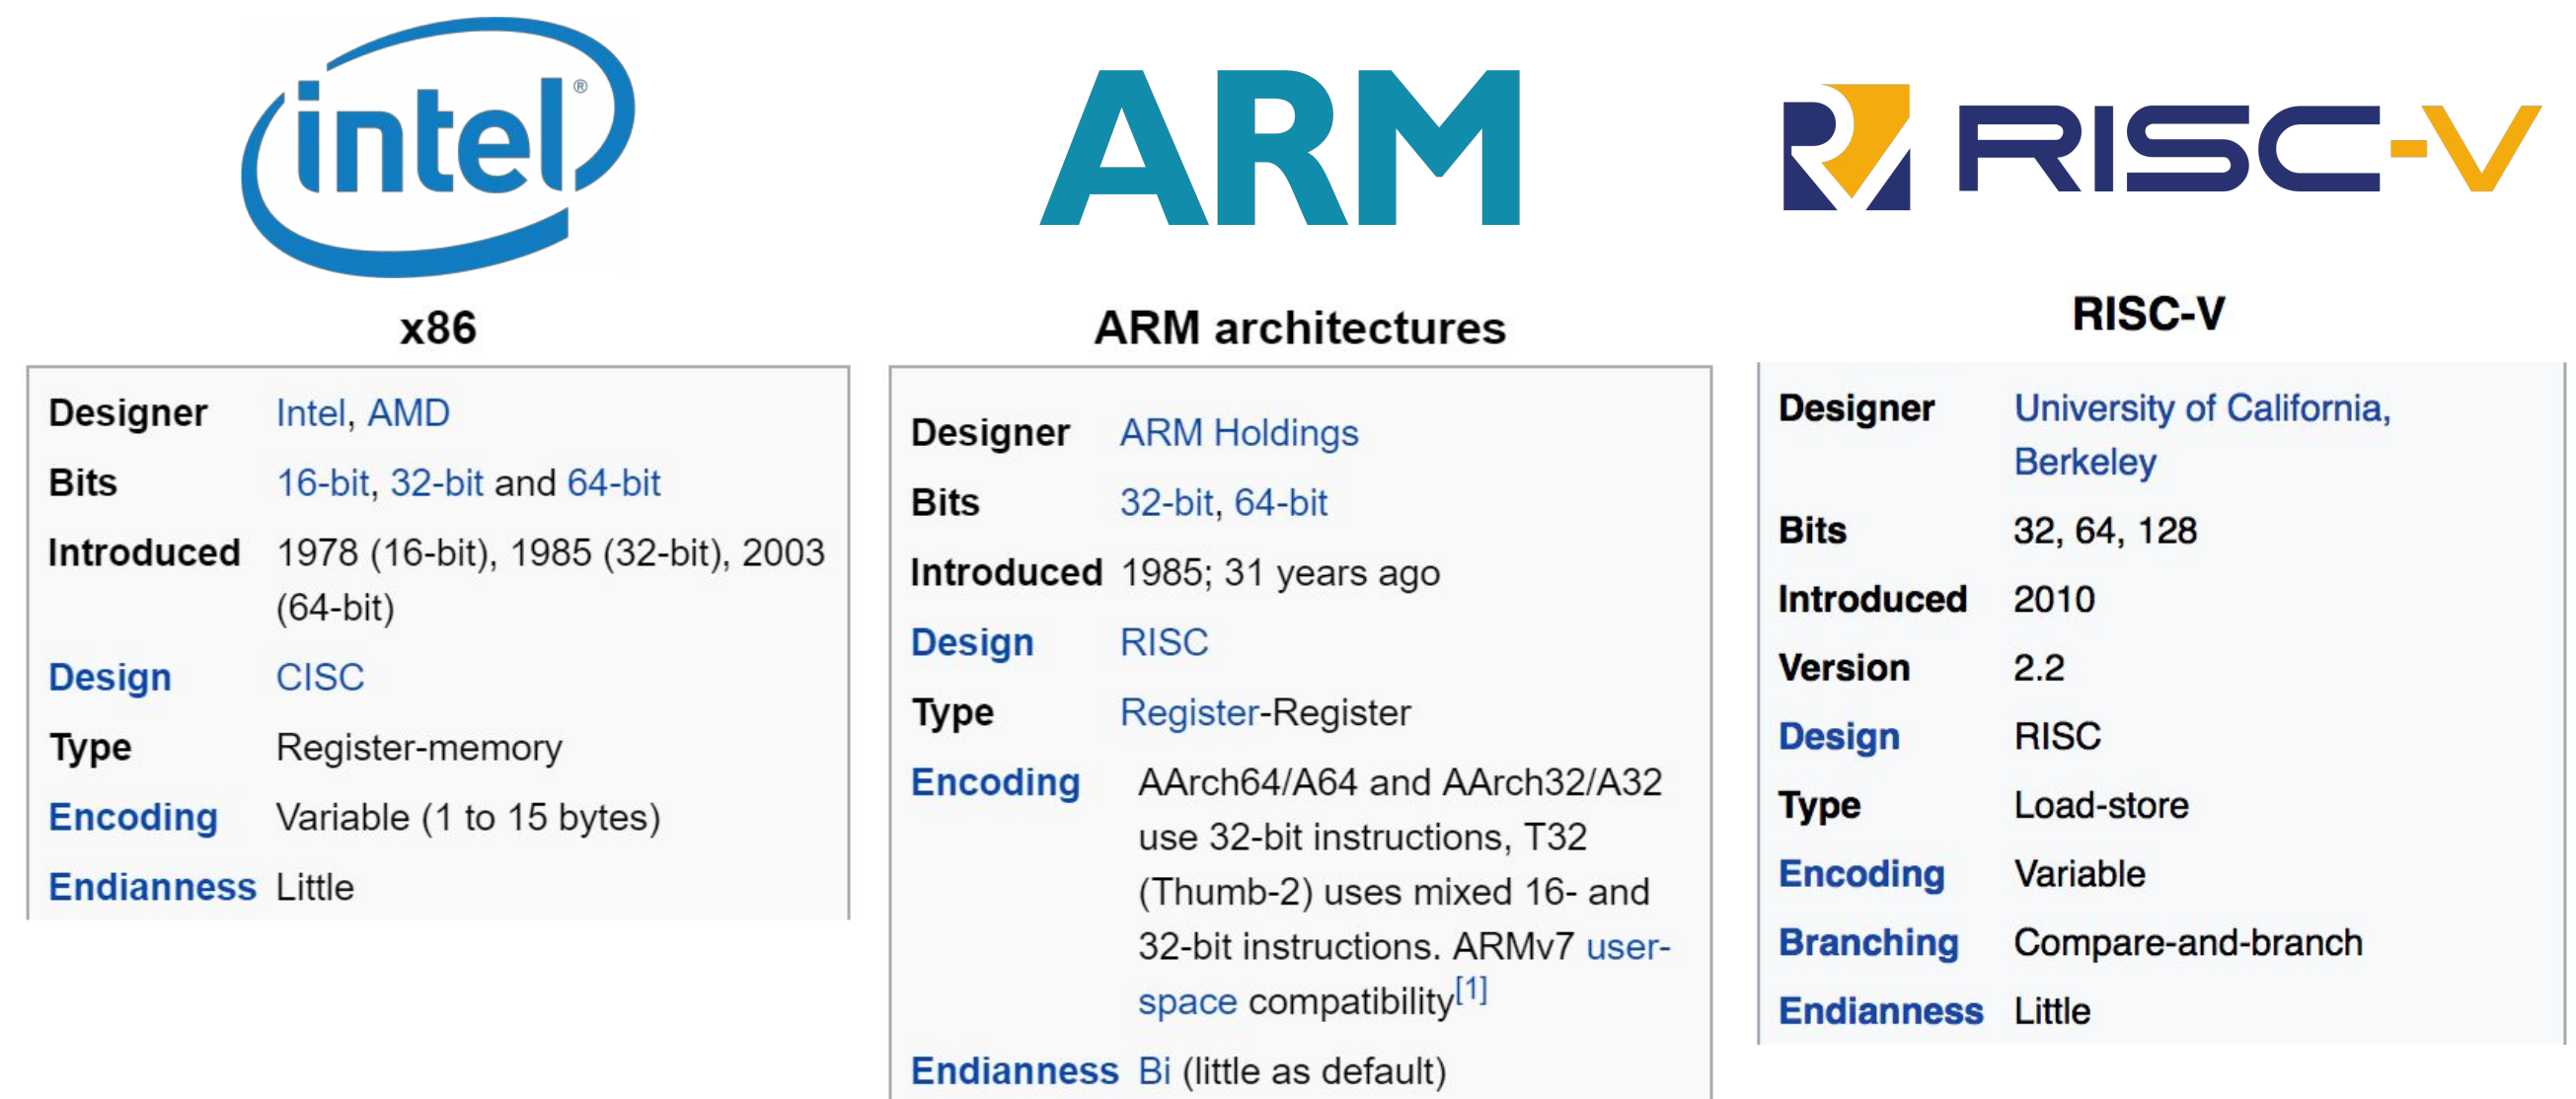
\includegraphics[width=0.65\linewidth]{mainstream-isas}
%		\caption{主流的ISAs$ _{[CS-61C Berkeley]} $}
	\end{figure}
	\pause
	
	\begin{figure}
		\centering
		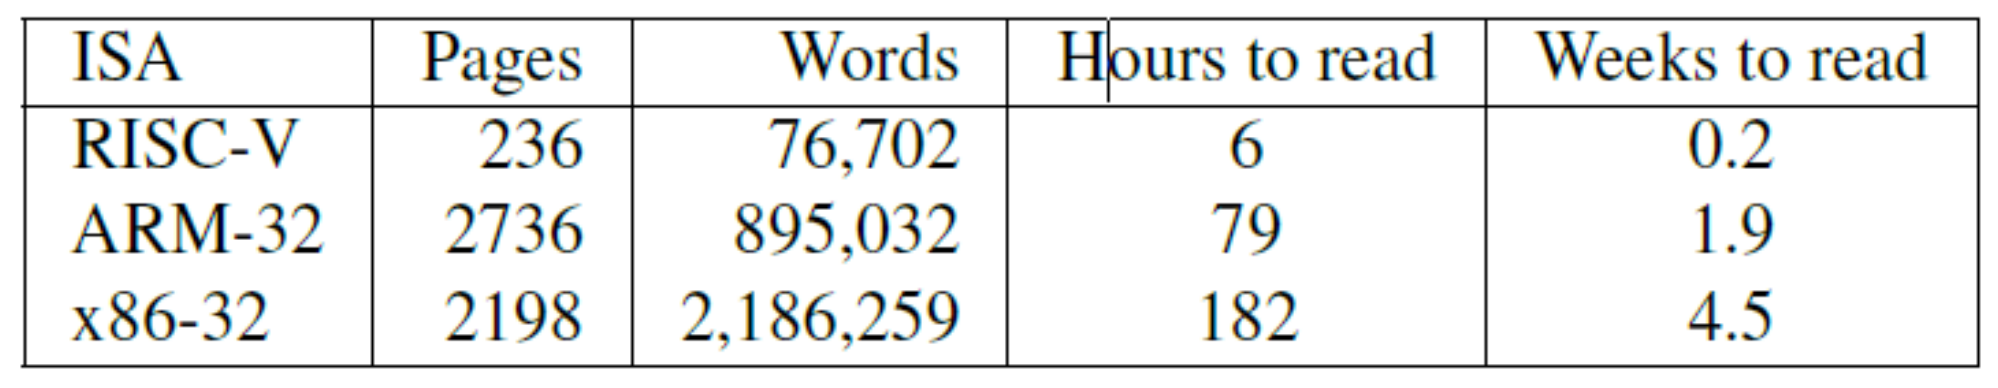
\includegraphics[width=0.6\linewidth]{x86-arm-rv-compare}
%		\caption{主流CPU指令集比较$ _{[Waterman 2017]} $}
	\end{figure}
	
	
	% x86指令集自诞生以来指令数量的增长。x86在1978年诞生时有80条指令,到2015年增长了16倍	
	
	% RISC-V的不同寻常之处,除了在于它是最近诞生的和开源的以外,还在于:和几乎所
	% 有以往的ISA不同,它是模块化的。它的核心是一个名为RV32I的基础ISA,运行一个完整
	% 的软件栈。RV32I是固定的,永远不会改变。这为编译器编写者,操作系统开发人员和汇
	% 编语言程序员提供了稳定的目标。模块化来源于可选的标准扩展,根据应用程序的需要,
	% 硬件可以包含或不包含这些扩展。	
	
\end{frame}

%------------------------------------------------

\begin{frame}
    \frametitle{提纲} 
    \tableofcontents 
\end{frame}

\subsection{RISC-V系统模式:概述}
\begin{frame}
    \frametitle{RISC-V系统模式:\small{概述}}
    %	\framesubtitle{隔离}
    
    \begin{figure}
        \centering
        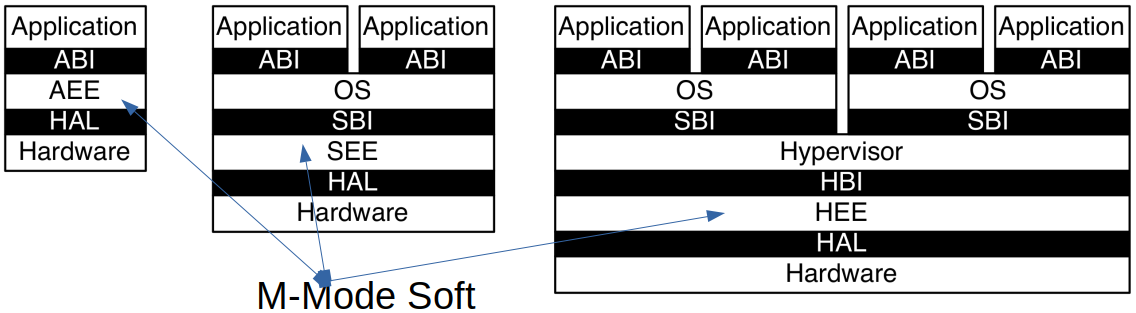
\includegraphics[width=0.6\linewidth]{rv-privil-arch}
        %	\caption{RISC-V特权架构}
    \end{figure}
    
    \begin{itemize}
        
        \item RISC-V系统模式即RISC-V的特权级模式
        \item 现代处理器一般具有多个特权级的模式
        \item 每一个特权级所能够执行的指令以及能够访问的处理器资源是不同的
        
    \end{itemize}
    
\end{frame}

%------------------------------------------------
\begin{frame}
    \frametitle{RISC-V系统模式:\small{概述}}
    %	\framesubtitle{隔离}
    
    \begin{figure}
        \centering
        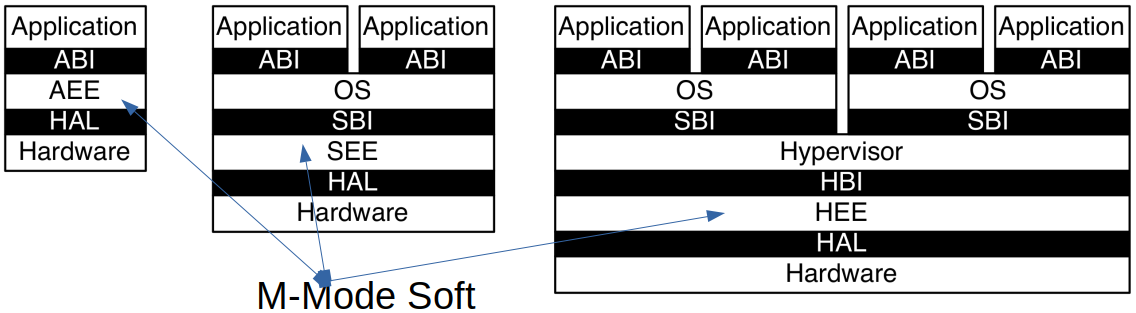
\includegraphics[width=0.6\linewidth]{rv-privil-arch}
        %	\caption{RISC-V特权架构}
    \end{figure}

    RISC-V系统模式:内核态特权级
    
    简单情况下:
    \begin{itemize}
        \item 用户态专门用来执行应用程序
        \item 内核态专门用来执行操作系统
        \item 内核态的操作系统具有完全的硬件控制能力
        
    \end{itemize}
    
\end{frame}
%------------------------------------------------

\begin{frame}
	\frametitle{RISC-V系统模式:\small{隔离}}
%	\framesubtitle{隔离}
	
	\begin{figure}
	\centering
	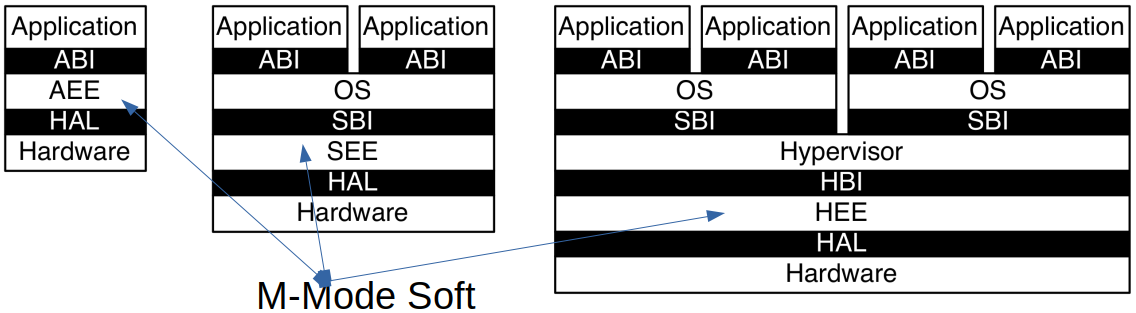
\includegraphics[width=0.9\linewidth]{rv-privil-arch}
%	\caption{RISC-V特权架构}
	\end{figure}

\begin{itemize}
	
	\item 不同软件层有清晰的硬件隔离
	\item AEE: Application Execution Environment
	\item ABI: Application Bianry Interface
	\item \textbf{MODE} -- \textbf{U}: User | \textbf{S}: Supervisor | \textbf{H}: Hypervisor | \textbf{M}: Machine

\end{itemize}

\end{frame}

%------------------------------------------------

\begin{frame}
		\frametitle{RISC-V系统模式:\small{模式组合}}
%		\framesubtitle{隔离}
\begin{table}[h]
%	\caption{RISC-V的特权模式组合}
 	\centering
 	\begin{tabular}{|c|c|l|c|l|}
 	\hline
	0 & 00 & User/Application & U \\\hline
	1 & 01 & Supervisor & S \\\hline
	2 & 10 & Hypervisor & H \\\hline
	3 & 11 & Machine & M \\\hline
   \end{tabular}
   \end{table}
\begin{itemize}
	
	\item M, S, U  for systems running Unix-like general operating systems
	%内核模式是指RV的哪种特权模式?
\end{itemize}


% \end{table}
\end{frame}

%------------------------------------------------

\begin{frame}
	\frametitle{RISC-V系统模式:\small{控制状态寄存器}}
%	\framesubtitle{隔离}

	\begin{itemize}
		\item 设置CSR(控制状态寄存器)实现隔离
		\begin{itemize}
			\item 防止应用程序访问设备和敏感的CPU寄存器
			\item 例如地址空间配置寄存器
		\end{itemize} 
	\end{itemize}

	\begin{itemize}
		\item 强制隔离以避免对整个系统的可用性/可靠性/安全影响
		\begin{itemize}
		\item 运行的程序通常是隔离的单元
		\item 防止恶意程序、病毒、木马破坏或监视应用程序或干扰操作系统	
			\begin{itemize}
			\item 读/写内存: mstatus/satp CSR
			\item 使用100%的CPU:mstatus/stvec CSR
%			\item 更改FD:??? CSR

			 	\item mstatus/satp/stvec CSR 页表异常处理

			\end{itemize}
		\end{itemize}
	\end{itemize}

\end{frame}
%------------------------------------------------
\begin{frame}
    \frametitle{RISC-V系统编程}
    \begin{itemize}
        \item 系统编程即据了解处理器的特权级架构,熟悉各个特权级能够访问的寄存器资源,内存资源,外设资源        
        \item 编写内核级代码,构造操作系统,支持应用程序执行
        \begin{itemize}
            \item 内存管理 \quad 进程调度
            \item 异常处理 \quad 中断处理
            \item 系统调用 \quad 外设控制
        \end{itemize}				
        \item 系统编程通常没有广泛用户编程库和方便的动态调试手段的支持
        \item 本课程的系统编程主要集中在RISC-V的S-Mode和U-Mode
    \end{itemize}
    
\end{frame}

%------------------------------------------------

\begin{frame}
    \frametitle{RISC-V系统编程:特权操作}
    \begin{itemize}
        \item 特权操作:包括特权指令以及相应的指令码和操作数       
        \item 指令码非常少:
        \begin{itemize}
            \item mret 机器模式返回 \quad sret 监管者模式返回
            \item wfi 等待中断 \quad \quad \quad \quad sfense.vma 虚拟地址屏障指令
        \end{itemize}				
        \item 很多功能通过控制状态寄存器(CSR:Control State Register)来实现
    \end{itemize}
    
\end{frame}

%------------------------------------------------
\begin{frame}
    \frametitle{RISC-V系统编程:M-Mode}
    \begin{itemize}
        \item M模式是RISC-V中hart(硬件线程,hardware thread)的最高权限模式       
        \item M模式下,hart对内存,I/O,启动和配置的底层功能有完全的使用权
        \item 标准RISC-V处理器都必须实现的权限模式
        \item M模式最重要的特性是拦截和处理中断和异常
        \begin{itemize}
            \item 异常:执行期间产生,访问无效的寄存器地址,或执行无效操作码的指令
            \item 中断:指令流异步的外部事件,中断,如时钟中断
        \end{itemize}				
        \item RISC-V要求实现精确异常:保证异常之前的所有指令都完整执行,后续指令都没有开始执行
    \end{itemize}
    
\end{frame}

%------------------------------------------------

\begin{frame}[plain]
    \frametitle{RISC-V系统编程:M-Mode:RISC-V中断机制}
    \begin{itemize}
        \item 中断是异步发生,是来自处理器外部的I/O设备的信号的结果。
        
        
        \item Timer可以稳定定时地产生中断
        \begin{itemize}
            \item 防止应用程序死占着CPU不放,让OS Kernel能得到执行权...
        \end{itemize}				
        
    \end{itemize}
    
    %	\begin{figure}
    \centering
    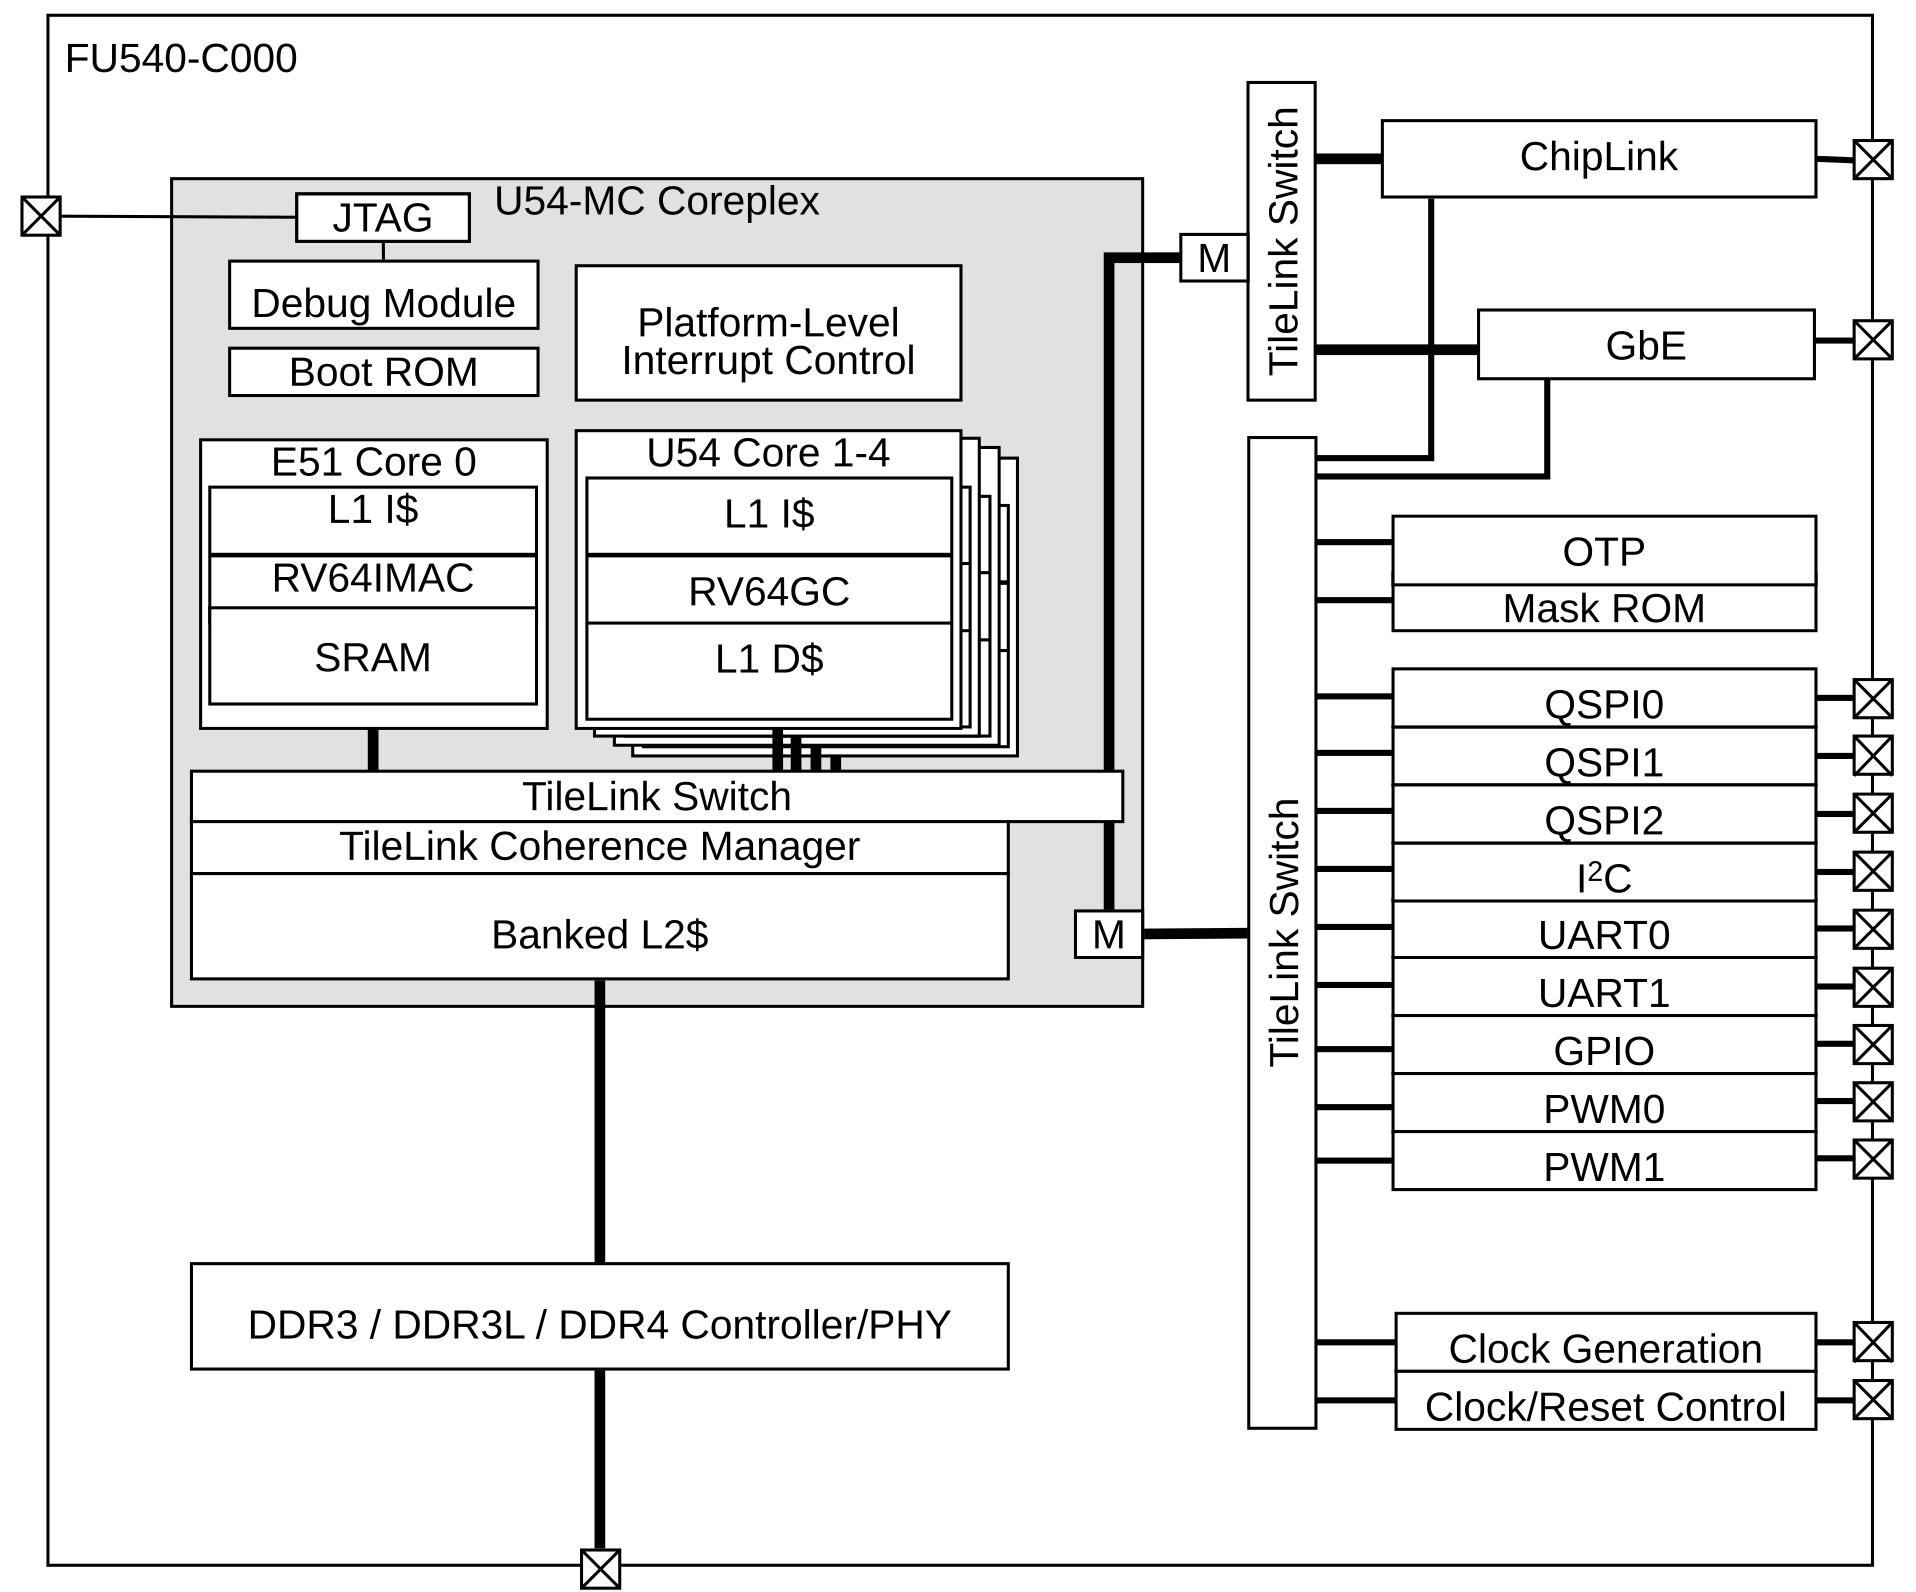
\includegraphics[width=0.5\linewidth]{fu540-top-block}
    %	\caption{RISC-V中断机制}
    %\end{figure}
    
\end{frame}

%------------------------------------------------

\begin{frame}
    \frametitle{RISC-V系统编程:M-Mode:RISC-V中断机制}
    \begin{itemize}
        \item 中断是异步发生,是来自处理器外部的I/O设备的信号的结果。
        
        
        \item Timer可以稳定定时地产生中断
        \begin{itemize}
            \item 防止应用程序死占着CPU不放,让OS Kernel能得到执行权...
            \item 由高特权模式下的软件获得CPU控制权
            \item 也可由高特权模式下的软件授权低特权模式软件处理中断
        \end{itemize}				
        
    \end{itemize}
    
    %	\begin{figure}
    \centering
    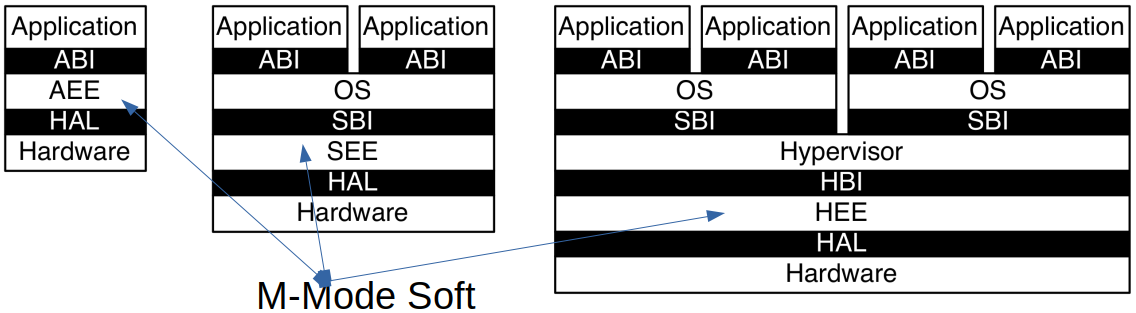
\includegraphics[width=0.7\linewidth]{rv-privil-arch}
    %	\caption{RISC-V中断机制}
    %\end{figure}
    
\end{frame}
%------------------------------------------------
\begin{frame}[plain]
    
    \begin{columns}
        \begin{column}{0.6\textwidth}
            
            \frametitle{RISC-V系统编程:S-Mode:虚拟内存}
            
            \begin{figure}
                \centering
                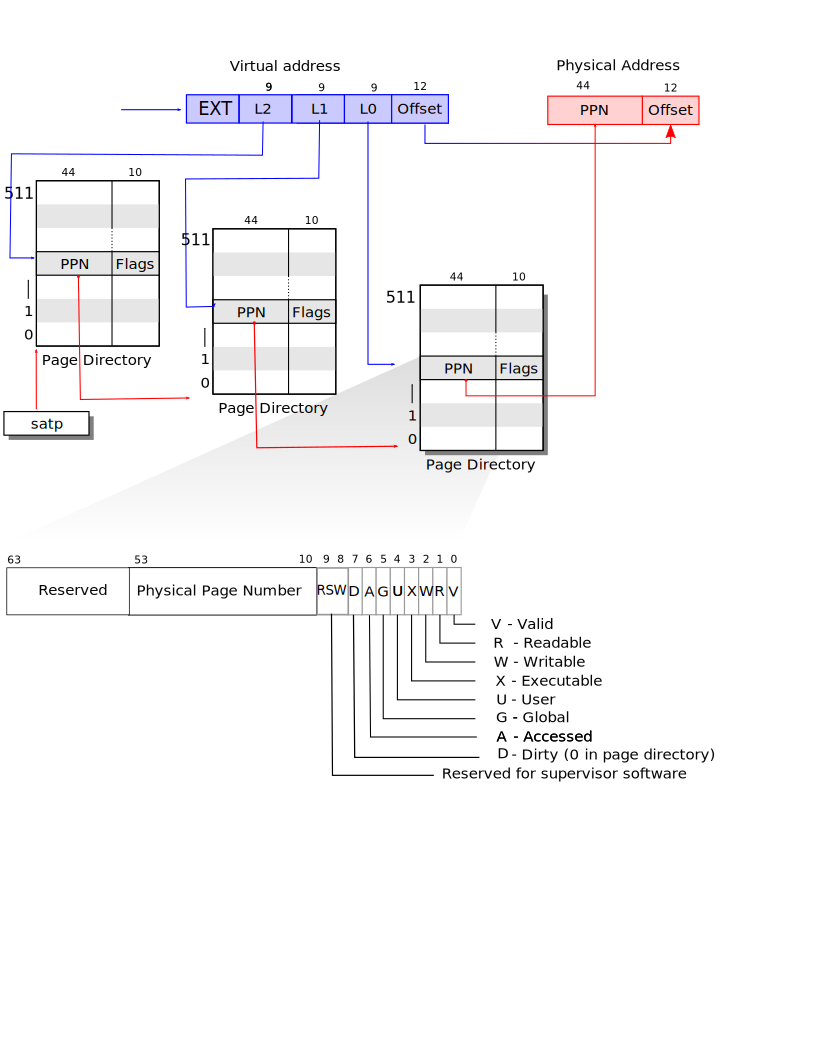
\includegraphics[width=0.7\linewidth]{riscv_pagetable}
                %		\caption{RISC-V虚拟内存}
            \end{figure}
            
        \end{column}
        
        \begin{column}{0.4\textwidth}
            
            \begin{itemize}
                \item 有虚拟内存的好处/坏处
                \begin{itemize}
                    \item 灵活的不连续内存分配
                    \item 多个运行程序的地址空间相互隔离/共享
                    \item 进一步隔离应用程序与OS内核
                    \item \textit{多了访问页表的开销} 
                \end{itemize} 
            \end{itemize}
            
        \end{column}
        
    \end{columns}
    
    
\end{frame}


%------------------------------------------------

\begin{frame}
    \frametitle{RISC-V系统编程:RISC-V的异常与中断}
    RISC-V的异常: 通过mcause寄存器的不同位来表示
    
    %	\begin{figure}
    \centering
    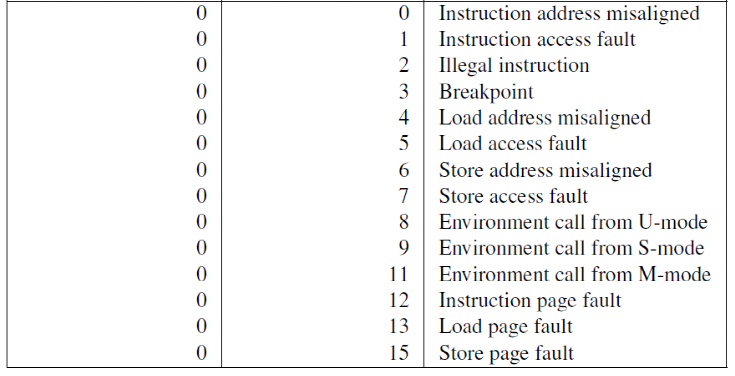
\includegraphics[width=0.9\linewidth]{rv-exception}
    %	\caption{RISC-V中断机制}
    %\end{figure}
    
\end{frame}

%------------------------------------------------

\begin{frame}
    \frametitle{RISC-V系统编程:RISC-V的异常与中断}
    RISC-V的中断: 通过mcause寄存器的不同位来表示
    
        \begin{itemize}
        \item 软件中断:通过向内存映射寄存器写入数据来触发,一个hart中断另外一个hart(处理器间中断)
        \item 时钟中断:hart的时间计数器寄存器mtime大于时间比较寄存器mtimecmp
        \item 外部中断:由中断控制器触发,大部分情况下的外设都会连到这个中断控制器
        
    \end{itemize}
    %	\begin{figure}
    \centering
    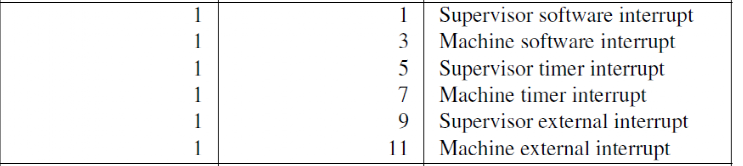
\includegraphics[width=0.8\linewidth]{rv-interrupt}
    %	\caption{RISC-V中断机制}
    %\end{figure}
    
\end{frame}

%------------------------------------------------

\begin{frame}
    \frametitle{RISC-V系统编程:RISC-V的系统调用}
    \begin{itemize}
    \item U-Mode下的应用程序不能够直接使用计算机的物理资源
    \item 环境调用异常:在执行ecall的时候发生,相当于系统调用
    \item 操作系统可以直接访问物理资源
    \item 如果应用程序需要使用硬件资源怎么办?

    \begin{itemize}
        \item 在屏幕上打印”hello world”
        \item 从文件中读入数据
    \end{itemize}	\pause			
    \item 通过系统调用从操作系统中获得服务
\end{itemize}

    
\end{frame}
%----------------------------------------------------------------------------------------
%------------------------------------------------

\begin{frame}
    \frametitle{RISC-V系统编程:思考题}

    \begin{itemize}
        \item 如何通过断点异常来实现调试器的断点调试功能?
        \item 如何实现单步跟踪?

    \end{itemize}
    
    
\end{frame}

%------------------------------------------------
\begin{frame}
\frametitle{提纲} % Table of contents slide, comment this block out to remove it
\tableofcontents % Throughout your presentation, if you choose to use \section{} and \subsection{} commands, these will automatically be printed on this slide as an overview of your presentation
\end{frame}

%----------------------------------------------------------------------------------------
\subsection{RISC-V系统编程:M模式}
\begin{frame}
    \frametitle{RISC-V系统编程:M模式下的异常处理}
    8个控制状态寄存器(CSR)是机器模式下异常处理的必要部分:part1
    \begin{itemize}
        \item mtvec(Machine Trap Vector):发生异常时处理器需要跳转到的地址
        \item mepc(Machine Exception PC):指向发生异常的指令
        \item mcause(Machine Exception Cause):发生异常的种类
        \item mie(Machine Interrupt Enable):处理器目前能处理和必须忽略的中断
                
    \end{itemize}
    
    
\end{frame}
%------------------------------------------------

\begin{frame}
    \frametitle{RISC-V系统编程:M模式下的异常处理}
    8个控制状态寄存器(CSR)是机器模式下异常处理的必要部分:part2
    \begin{itemize}
        \item mip(Machine Interrupt Pending):正准备处理的中断
        \item mtval(Machine Trap Value):附加信息:地址异常中出错的地址,非法指令异常的指令等
        \item mscratch(Machine Scratch):暂时存放一个字大小的数据
        \item mstatus(Machine Status):机器的状态
        
    \end{itemize}
    
    
\end{frame}
%------------------------------------------------

\begin{frame}
    \frametitle{RISC-V系统编程:M模式下的异常处理}
     mstatus控制状态寄存器
    \begin{itemize}
        \item 在仅有机器模式,且没有F和V扩展的简单处理器中,有效的域只有全局使能,MIE和MPIE(它在异常发生后保存MIE的旧值)
        \item 处理器在 M 模式下运行时,只有在全局中断使能位 mstatus.MIE 置 1 时才会产生中断
        
    \end{itemize}
    
    \begin{figure}
    \centering
    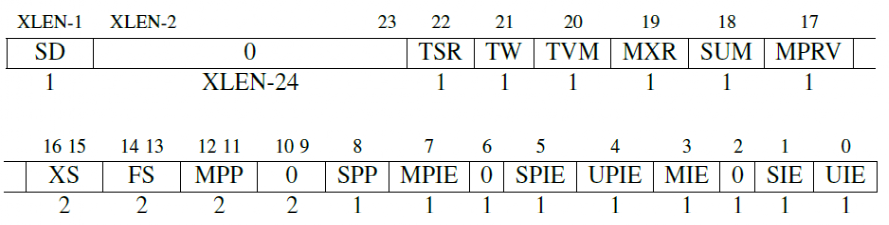
\includegraphics[width=0.8\linewidth]{rv-mstatus}
    \caption{mstatus寄存器}
    \end{figure}
    
\end{frame}

%------------------------------------------------

\begin{frame}
    \frametitle{RISC-V系统编程:M模式下的中断相关寄存器}
    \begin{itemize}
        \item M模式中断寄存器。它们是宽为 XLEN 位的读/写寄存器,用于保存待处理的中断(mip)和中断使能位(mie)CSR。
        \item 只有与 mip 中的位对应的低权限软件中断(USIP,SSIP)、时钟中断(UTIP,STIP)和外部中断(UEIP,SEIP)的位才能通过该 CSR 的地址写入;其余的位是只读的。
    \end{itemize}   
    \begin{figure}
        \centering
        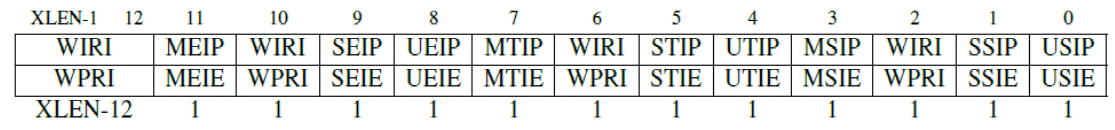
\includegraphics[width=0.9\linewidth]{rv-mie-mip}
        \caption{mie \&  mip寄存器}
    \end{figure}
\end{frame}

%------------------------------------------------

\begin{frame}
    \frametitle{RISC-V系统编程:M模式下的中断相关寄存器}
    \begin{itemize}
        \item 机器模式和监管模式异常向量(trap-vector)基地址寄存器(mtvec 和 stvec)CSR。他们是位宽为XLEN 的读/写寄存器,用于保存异常向量的配置,包括向量基址(BASE)和向量模式(MODE)。BASE 域中的值必须按 4 字节对齐。MODE = 0 表示所有异常都把 PC 设置为 BASE。MODE = 1 会在异步中断时将 PC 设置为(base+(4 * cause))。
    \end{itemize}   
    \begin{figure}
        \centering
        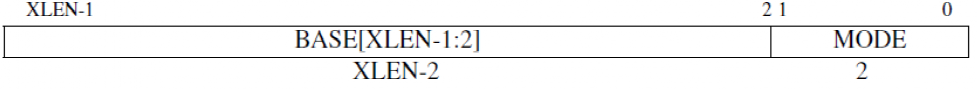
\includegraphics[width=0.9\linewidth]{rv-tvec}
        \caption{mtvec  \& stvec寄存器}
    \end{figure}
\end{frame}

%------------------------------------------------

\begin{frame}
    \frametitle{RISC-V系统编程:M模式下的中断相关寄存器}
    \begin{itemize}
        \item 机器模式和监管模式 cause(mcause 和 scause)CSR。当处理发生异常时,CSR 中被写入一个指示导致异常的事件的代码。如果异常由中断引起,则置上中断位。“异常代码”字段包含指示最后一个异常的代码。
    \end{itemize}   
    \begin{figure}
        \centering
        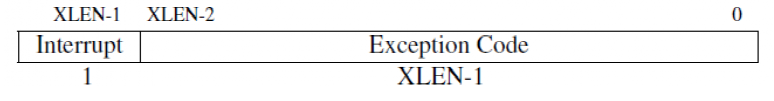
\includegraphics[width=0.9\linewidth]{rv-cause}
        \caption{mcause  \& scause寄存器}
    \end{figure}
\end{frame}
%------------------------------------------------

\begin{frame}
    \frametitle{RISC-V系统编程:M模式下的异常处理}
    硬件执行内容
    \begin{itemize}
        \item 异常指令的PC被保存在mepc中,pc被置为mtvec。(对于同步异常,mepc指向导致异常的指令;对于中断它指向中断处理后应该恢复执行的位置)
        \item 根据异常来源设置mcause,并将mtval设置为出错的地址或者其它使用特定异常的信息字
        \item 把控制状态寄存器mstatus中的MIE位置零以禁用中断,并把先前的MIE值保留到MPIE中
        \item 发生异常前的权限模式保留在mstatus的MPP域中,再把权限模式更改为M
        
    \end{itemize}
    
%    \begin{figure}
        \centering
        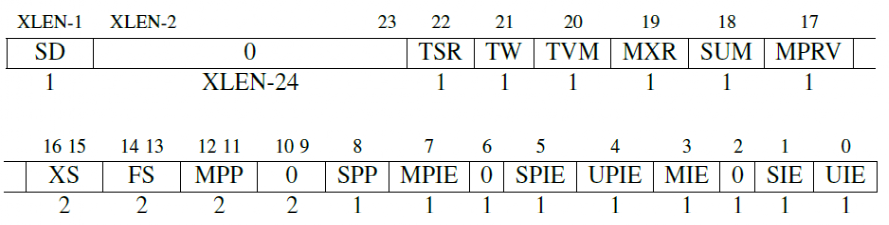
\includegraphics[width=0.6\linewidth]{rv-mstatus}
%        \caption{mstatus寄存器}
%    \end{figure}
    
\end{frame}

%------------------------------------------------

\begin{frame}
    \frametitle{RISC-V系统编程:M模式下的异常处理}
    软件执行内容(如时钟中断)
    \begin{itemize}
        \item 保存上下文:保存各种寄存器到异常处理程序用到的特定内存(栈)中
        \item 根据异常来源进行异常或中断的处理(如改mtimecmp)
        \item mie[7]对应于M模式中的时钟中断,mip指示当前待处理的中断
        \item 如果 mstatus.MIE = 1,mie[7] = 1,且 mip[7] = 1,则可处理机器的时钟中断
        \item 恢复上下文:恢复各种寄存器,把mstatus中的MPIE等写到MIE等中
        \item 执行 mret 回到被打断的地方继续执行
        
    \end{itemize}
    
    %    \begin{figure}
    \centering
    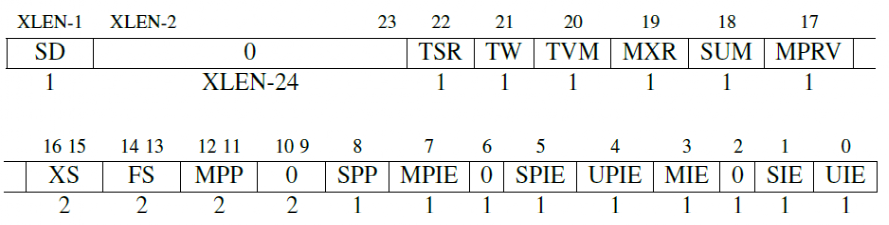
\includegraphics[width=0.6\linewidth]{rv-mstatus}
    %        \caption{mstatus寄存器}
    %    \end{figure}
    
\end{frame}

%------------------------------------------------

\begin{frame}
    \frametitle{RISC-V系统编程:M模式下的异常处理}
    软件执行内容:可抢占式异常处理
    \begin{itemize}
        \item 在处理异常的过程中转到处理更高优先级的中断
        \item mepc, mcause, mtval,mstatus,mscratch等寄存器只有一个副本
        \item 可抢占的中断处理程序在启动中断之前把这些寄存器保存到内存中的栈
        \item 然后再退出之前,禁用中断并从栈中恢复寄存器
        
    \end{itemize}
    
    %    \begin{figure}
    \centering
    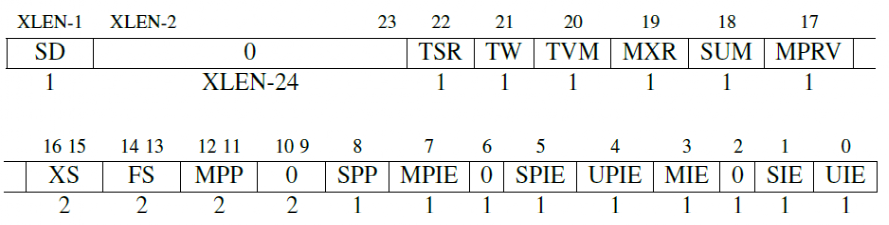
\includegraphics[width=0.6\linewidth]{rv-mstatus}
    %        \caption{mstatus寄存器}
    %    \end{figure}
    
\end{frame}
%------------------------------------------------

\begin{frame}
    \frametitle{RISC-V系统编程:M模式下的隔离}
    特权指令隔离
    \begin{itemize}
        \item 通过设置用户模式(不可信的代码)来阻止用户执行特权指令(例如mret)和访问控制状态寄存器(如mstatus)
        \item 用户模式拒绝执行这些指令,会产生非法指令异常
        \item mstatus.MPP设置为U,然后执行mret指令,软件可以从M模式进入U模式
        \item 如果在U模式下发生异常,则把控制权移交给M模式
        
    \end{itemize}
    
    %    \begin{figure}
    \centering
    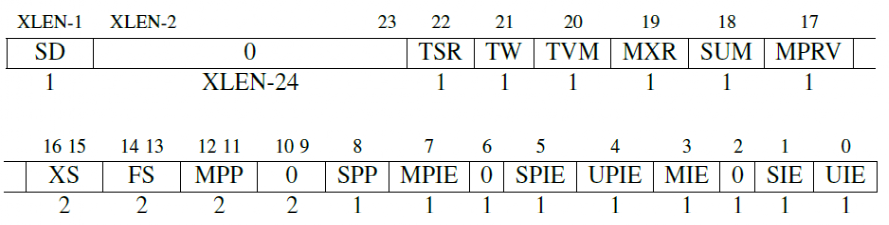
\includegraphics[width=0.6\linewidth]{rv-mstatus}
    %        \caption{mstatus寄存器}
    %    \end{figure}
    
\end{frame}

%------------------------------------------------

\begin{frame}
    \frametitle{RISC-V系统编程:M模式下的隔离}
    内存隔离
    \begin{itemize}
        \item 实现M和U模式,物理内存保护(PMP:Physical Memory Protection),M模式指定U模式可以访问的内存地址
        \item pmpaddr0 ~ pmpaddrN地址寄存器,pmpcfg配置寄存器,地址从小到大排列
        \item 如果地址大于等于 PMP 地址 i,但小于 PMP 地址 i+1,则 PMP i+1 的配置寄存器决定该访问是否可以继续,如果不能将会引发访问异常。
        \item A: available, X: executable, W: writable, R: readable,L: lock
        
    \end{itemize}
    
    %    \begin{figure}
    \centering
    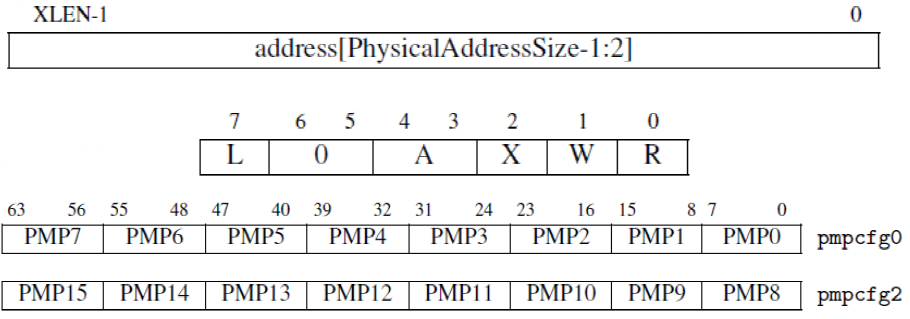
\includegraphics[width=0.6\linewidth]{rv-pmp}
    %        \caption{mstatus寄存器}
    %    \end{figure}
    
\end{frame}
%------------------------------------------------
\begin{frame}
    \frametitle{提纲} 
    \tableofcontents 
\end{frame}

\subsection{RISC-V系统编程:S模式}
%------------------------------------------------

\begin{frame}
    \frametitle{RISC-V系统编程:S模式下的隔离}
    \begin{itemize}
        \item S模式比U模式权限更高,但是比M模式权限低
        \item S模式下运行的软件不能使用M模式的CSR和指令,并受到PMP的限制
        \item 支持基于页面的虚拟内存
        
    \end{itemize}
    
\end{frame}
%------------------------------------------------


\begin{frame}
    \frametitle{RISC-V系统编程:S模式下的异常处理}
    \begin{itemize}
        \item 默认情况下,所有的异常都使得控制权移交到M模式的异常处理程序
        \item M模式的异常处理程序可以将异常重新导向S模式,但是这些额外的操作会减慢异常的处理速度
        \item RISC-V提供一种异常委托机制,通过该机制可以选择性地将中断和同步异常交给 S 模式处理,而完全绕过 M 模式
        
    \end{itemize}
   
    
\end{frame}
%------------------------------------------------

%------------------------------------------------

\begin{frame}
    \frametitle{RISC-V系统编程:异常委托寄存器}
    \begin{itemize}
        \item mideleg (Machine Interrupt Delegation)CSR控制将哪些中断委托给S模式处理
        \item 与mip和mie一样,mideleg中的每个为对应一个异常
        \begin{itemize}
            \item 如mideleg[5]对应于S模式的时钟中断,如果把它置位,S模式的时钟中断将会移交S模式的异常处理器程序,而不是M模式的异常处理程序
            \item 委托给S模式的任何中断都可以被S模式的软件屏蔽。sie(Supervisor Interrupt Enable)和sip(Supervisor Interrupt Pending)CSR是S模式的控制状态寄存器,是mie和mip的子集。这两个寄存器和M模式下有相同的布局。sie和sip中只有与由mideleg委托的中断对应的位才能读写,没有委派的中断对应位总是0    
        \end{itemize}
        
    \end{itemize}
    
\end{frame}

%------------------------------------------------

\begin{frame}
    \frametitle{RISC-V系统编程:异常委托寄存器}
    \begin{itemize}
        \item M模式还可以通过medeleg CSR将同步异常委托给S模式。
        \item 另外,发生异常时控制权都不会移交给权限更低的模式
        \begin{itemize}
            \item 例如medeleg[15]会把store page fault委托给S模式
            \item M模式下发生的异常总是在M模式下处理
            \item S模式下发生的异常总是在M或S模式下处理
            \item 上述两种模式发生的异常不会由U模式处理(除非有U模式中断处理机制)
        \end{itemize}
        
    \end{itemize}
    
\end{frame}
%------------------------------------------------

\begin{frame}
    \frametitle{RISC-V系统编程:S模式的CSR寄存器}

    \begin{itemize}
        \item S模式有异常处理CSR:sepc, stvec, scause, sscratch, stval和sstatus,与M模式的寄存器相对应
        \item sret返回指令和mret指令也类似,但是它作用于S模式的异常处理CSR
        
    \end{itemize}
    
        \begin{figure}
    \centering
    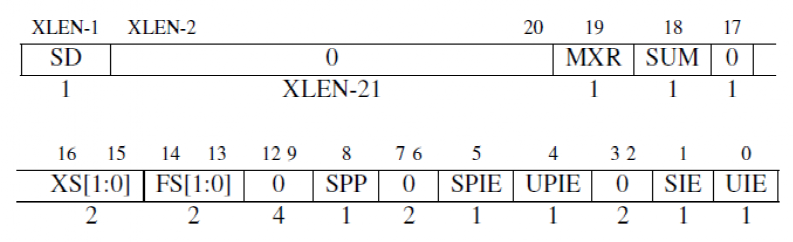
\includegraphics[width=0.6\linewidth]{rv-sstatus}
            \caption{sstatus寄存器}
        \end{figure}
    
\end{frame}

%------------------------------------------------

\begin{frame}
    \frametitle{RISC-V系统编程:S模式下的中断相关寄存器}
    \begin{itemize}
        \item S模式中断寄存器。它们是宽为 XLEN 位的读/写寄存器,用于保存待处理的中断(sip)和中断使能位(sie)CSR。
    \end{itemize}   
    \begin{figure}
        \centering
        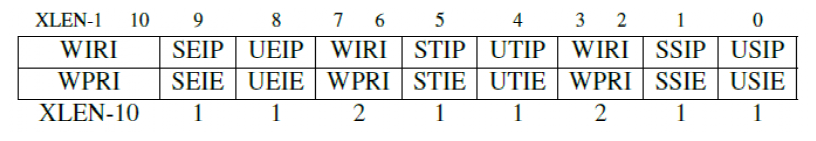
\includegraphics[width=0.9\linewidth]{rv-sie-sip}
        \caption{sie  \& sip寄存器}
    \end{figure}
\end{frame}

%------------------------------------------------

\begin{frame}
    \frametitle{RISC-V系统编程:S模式下的中断相关寄存器}
    \begin{itemize}
        \item 机器模式和监管模式异常向量(trap-vector)基地址寄存器(mtvec 和 stvec)CSR。他们是位宽为XLEN 的读/写寄存器,用于保存异常向量的配置,包括向量基址(BASE)和向量模式(MODE)。BASE 域中的值必须按 4 字节对齐。MODE = 0 表示所有异常都把 PC 设置为 BASE。MODE = 1 会在异步中断时将 PC 设置为(base+(4 * cause))。
    \end{itemize}   
    \begin{figure}
        \centering
        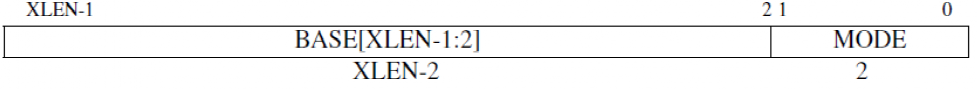
\includegraphics[width=0.9\linewidth]{rv-tvec}
        \caption{mtvec  \& stvec寄存器}
    \end{figure}
\end{frame}

%------------------------------------------------

\begin{frame}
    \frametitle{RISC-V系统编程:S模式下的中断相关寄存器}
    \begin{itemize}
        \item 机器模式和监管模式 cause(mcause 和 scause)CSR。当处理发生异常时,CSR 中被写入一个指示导致异常的事件的代码。如果异常由中断引起,则置上中断位。“异常代码”字段包含指示最后一个异常的代码。
    \end{itemize}   
    \begin{figure}
        \centering
        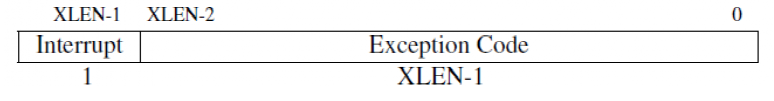
\includegraphics[width=0.9\linewidth]{rv-cause}
        \caption{mcause  \& scause寄存器}
    \end{figure}
\end{frame}
%------------------------------------------------
%------------------------------------------------

\begin{frame}
    \frametitle{RISC-V系统编程:S模式的异常处理}
     硬件执行内容
     
     hart接受了异常,并需要委派给S模式,那么硬件会作为一个原子操作完成下面的状态转换
    \begin{itemize}
        \item 发生异常的指令PC被存入sepc, 且PC被设置为stvec
        \item scause根据异常设置类型,stval被设置为出错的地址或者异常相关信息字
        \item 把sstatus CSR中的SIE置零,屏蔽中断,且SIE之前的值被保存在SPIE中
        \item 发生例外前的特权模式被保存在sstatus的SPP域,然后设置当前特权模式为S模式
        
    \end{itemize}
        \centering
    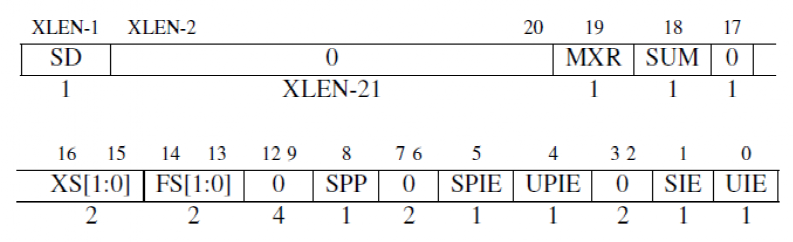
\includegraphics[width=0.6\linewidth]{rv-sstatus}
\end{frame}

%------------------------------------------------

\begin{frame}
    \frametitle{RISC-V系统编程:S模式的异常处理}
    
    相关指令
    \begin{itemize}
        \item ecall:触发中断,进入更高一层的中断处理流程之中。用户态进行系统调用进入内核态中断处理流程,内核态进行 SBI 调用进入机器态中断处理流程,使用的都是这条指令。
        \item sret:从内核态返回用户态,同时将 pc 的值设置为 sepc。(如果需要返回到 sepc 后一条指令,就需要在 sret 之前修改 sepc 的值)
        \item ebreak:触发一个断点。
        \item mret:从机器态返回内核态,同时将 pc 的值设置为 mepc。
        
    \end{itemize}
%    \centering
%    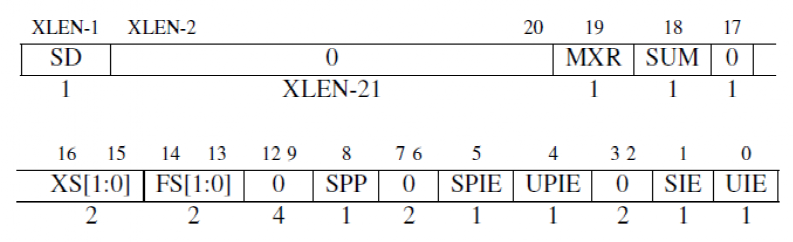
\includegraphics[width=0.6\linewidth]{rv-sstatus}
\end{frame}

%------------------------------------------------

\begin{frame}
    \frametitle{RISC-V系统编程:S模式的异常处理}
    
    操作CSR
    \begin{itemize}
        \item 只有一系列特殊的指令(CSR Instruction)可以读写 CSR。尽管所有模式都可以使用这些指令,用户态只能只读的访问某几个寄存器。
        \item 为了让操作 CSR 的指令不被干扰,许多 CSR 指令都是结合了读写的原子操作。

        
    \end{itemize}
    %    \centering
    %    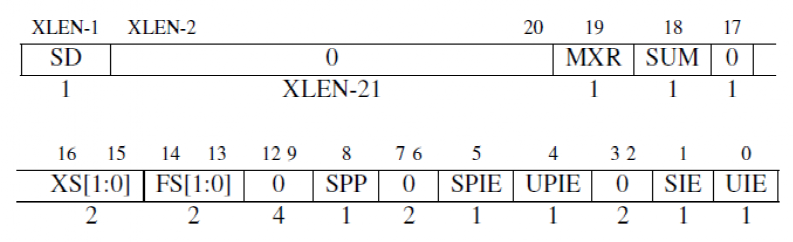
\includegraphics[width=0.6\linewidth]{rv-sstatus}
\end{frame}

%------------------------------------------------

\begin{frame}
    \frametitle{RISC-V系统编程:S模式的异常处理}
    
    操作CSR
    \begin{itemize}
        \item csrrw dst, csr, src(CSR Read Write):同时读写的原子操作,将指定 CSR 的值写入 dst,同时将 src 的值写入 CSR。
        \item csrr dst, csr(CSR Read):读取一个 CSR 寄存器。
        \item csrw csr, src(CSR Write):仅写入一个 CSR 寄存器。
        \item csrc(i) csr, rs1(CSR Clear):将 CSR 寄存器中指定的位清零,csrc 使用通用寄存器作为 mask,csrci 则使用立即数。
        \item csrs(i) csr, rs1(CSR Set):将 CSR 寄存器中指定的位置 1,csrc 使用通用寄存器作为 mask,csrci 则使用立即数。
    \end{itemize}
    %    \centering
    %    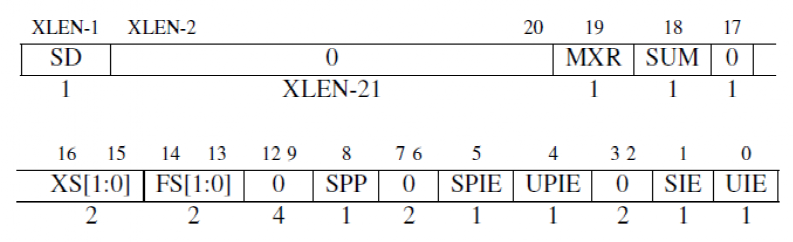
\includegraphics[width=0.6\linewidth]{rv-sstatus}
\end{frame}

%------------------------------------------------
%
%\begin{frame}
%    \frametitle{RISC-V系统编程:小结}
%    
%    \begin{itemize}
%        \item 所有的标准的RISC-V处理器都会实现M模式,这个模式使用尽可能少的硬件来实现对于异常和中断的支持,实现用户程序和操作系统的隔离,M模式适合需要一定保护的嵌入式操作系统
%        \item 在M模式之上RISC-V也定义了S模式,打开页式内存管理,支持虚拟内存的内存管理方式
%        \item 我们需要了解M模式,掌握S模式
%    \end{itemize}
%    %    \centering
%    %    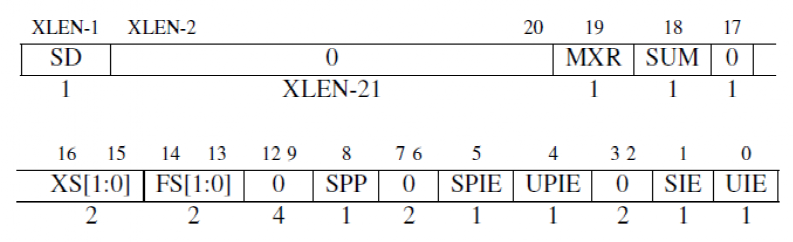
\includegraphics[width=0.6\linewidth]{rv-sstatus}
%\end{frame}
%%------------------------------------------------
\begin{frame}
    \frametitle{小结}
    \begin{itemize}
        \item 了解RISC-V的M-Mode和S-Mode的特征
        \item 了解系统软件在M-Mode和S-Mode下如何访问控制计算机系统
        \item 了解如何在M-Mode<-->S-Mode<-->U-Mode之间进行切换
    \end{itemize}
\end{frame}
%------------------------------------------------
\end{document}
